\appendixchapter{More on top quarks}

%##############################################
\section{Polarization in top quark pair production}
%##############################################


Similar to the study of the $\mathrm{W}$ boson helicity fractions in top quark decays, the polarization of the top quarks arising in pair production can be analyzed by decomposing the \ttbar cross section as a function of the polarization angles. One finds

\begin{align}
\frac{\mathrm{d}^{2}\sigma}{\sigma\cdot\mathrm{d}\cos\theta_{\mathrm{t}X}^\star~\mathrm{d}\cos\theta_{\bar{\mathrm{t}}X^\prime}^\star}=\frac{1}{4}\Big(1&+\mathrm{P}_\mathrm{t}\,\alpha_{X}\,\cos\theta_{\mathrm{t}X}^\star+\mathrm{P}_{\bar{\mathrm{t}}}\,\alpha_{X^\prime}\,\cos\theta_{\bar{\mathrm{t}}X^\prime}^\star \nonumber \\
&-\mathrm{C}\,\alpha_{X}\alpha_{X^\prime}\,\cos\theta_{\mathrm{t}X}^\star \cos\theta_{\bar{\mathrm{t}}X^\prime}^\star\Big) \label{eq:theory-ttbar-correlation}
\end{align}

where $\mathrm{P}_\mathrm{t}$ and $\mathrm{P}_{\bar{\mathrm{t}}}$ denote the polarization fractions and $\mathrm{C}$ the $\mathrm{t\bar{t}}$ spin correlation. In the helicity basis, the angles are taken between the momenta of the leptons~($X=\ell^{\rmplus}\,/\,X^\prime=\ell^{\rmminus}$) in the corresponding $\mathrm{t}/\bar{\mathrm{t}}$ rest frames and the momenta of the $\mathrm{t}/\bar{\mathrm{t}}$ in the $\ttbar$ \gls{zmf} respectively. Since the top quarks are produced isotropic at \gls{lo}, only a small net polarization of $\mathrm{P}_\mathrm{t}=-\mathrm{P}_{\bar{\mathrm{t}}}\approx0.3\%$ for $m_\mathrm{t\bar{t}}>2m_\mathrm{t}$ from electroweak higher order corrections is expected~\cite{Bernreuther:2010ny,Bernreuther:2013aga}. However, the spins of two top quarks within a pair are linked through the $\mathrm{g\mathrm{t}\bar{\mathrm{t}}}$ vertex yielding a large correlation between them~\cite{Mahlon:2010gw}. The correlation depends on the boost of the top quarks with respect to their \gls{zmf} and amounts to $C\approx32\%$ for $m_\mathrm{t\bar{t}}>2m_\mathrm{t}$ at $8~\TeV$~\cite{Bernreuther:2013aga}. Experimentally, the azimuthal $\Delta\phi$ angle between the two leptons in the laboratory frame is sometimes studied instead of the helicity angle. This observable has the advantage that the whole \ttbar system does not need to be reconstructed which involves finding solutions for the two unknown neutrino momenta while matching the two jets with the two leptons to setup two top quark decay chains\footnote{Kinematic fitting is sometimes deployed to solve this problem using the invariant mass of the intermediate top quarks and $\mathrm{W}$~bosons as constraints.}. The amount of correlation cannot be easily extracted from the $\Delta\phi$ distribution directly since its functional form does not resemble Eq.~\ref{eq:theory-ttbar-correlation}. However this observable is sensitive enough to test the presence of \ttbar correlation and to distinguish it from a potential \gls{bsm} scenario without correlation.


%##############################################
\section{Mass definitions}
%##############################################

Quarks cannot be observed freely at low energies because of strong interactions. Hence, the concept of mass for a quark needs to be defined through renormalization. The top quark is however special since it can be treated as a nearly free particle around and beyond the electroweak energy scale nonetheless. This leads to two common definitions of its mass which are described in the following. It is important to know which definition is used when comparing theoretical predictions to experimental data or even attempting to infer the ``mass'' from data itself.

The general problem arises from higher order corrections to the ``bare'' quark propagator as depicted in Fig.~\ref{fig:theory-quark-selfenergy}. 

\myfigure{\label{fig:theory-quark-selfenergy}Feynman diagrams at \gls{lo} and beyond contributing to the quark propagator.}{
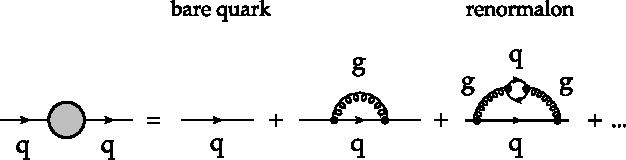
\includegraphics[scale=0.75]{figures/theory/quark_selfenergy.pdf}
}

These result in corrections which are absorbed into the mass definition using the concept of renormalization. The procedure is similar to the running strong coupling constant as briefly described in Sec.~\ref{sec:theory-qcd}. The ``bare'' quark propagator is modified after renormalization as

\begin{equation}
\frac{i}{\gamma_{\mu}p^{\mu}-m_\mathrm{bare}}\quad\Rightarrow\quad\frac{i}{\gamma_{\mu}p^{\mu}-m_\mathrm{bare}+\Sigma(p,m_\mathrm{bare},\mu)}
\end{equation}

where $m_\mathrm{bare}$ denotes the bare mass of a quark which is however unphysical and just a parameter in the Lagrangian. The function $\Sigma(p,m_\mathrm{bare},\mu)$ is called ``self-energy'' and contains finite corrections but also divergent terms where the later arise from the used regularization procedure\footnote{Dimensional regularization with $\epsilon=(4-d)/2$ leads to counterterms with $1/\epsilon$ divergences.}. It depends on the renormalization scale $\mu$ beyond which higher order corrections have been absorbed.

For the top quark, a common scheme is the on-shell renormalization. Here, one requires $\Sigma(p)=0$ and $\mathrm{d}\Sigma/\mathrm{d}p=0$ for $p=m$ which defines $m$ as the pole mass. However, this scheme is normally only suited for particles which are free at low energies like the leptons. For the top quark, an additional problem in the calculation of the self-energy arises from special diagrams called ``renormalons'' which feature vacuum polarization bubbles~(see last diagram in Fig.~\ref{fig:theory-quark-selfenergy}). These lead to an ambiguity on the order of $\Lambda_\mathrm{QCD}\approx200~\MeV$ in the top-quark pole mass definition\footnote{Technically, this ambiguity stems from the chosen path of integration around the singularities from the renormalons~\cite{Smith:1996xz}.}. Despite this, one usually refers to the pole mass as the top quark mass which is also adopted in this thesis. However, since this level of precision is nearly approached in measurements of the top quark mass, the ambiguity has to be understood further or one should move to other schemes instead~\cite{Smith:1996xz}.

The other common renormalization scheme is the \glsreset{msbar}\gls{msbar}. Here, only the divergent terms within the self-energy are absorbed into the mass definition. The mass will therefore depend explicitly on the renormalization scale. However, this allows to define also the mass of quarks at very low energies. In literature, this scheme is commonly used for the light quarks~\cite{Olive:2016xmw}. For the top quark, a difference of

\begin{equation}
m_\mathrm{pole}^\mathrm{t}-m_{\gls{msbar}}^\mathrm{t}(\mu)=173.5~\GeV-163.1~\GeV=10.4~\GeV
\end{equation}

has been calculated at \gls{nnlo} in \gls{qcd} between the pole and \gls{msbar} mass definitions for $\mu=m_\mathrm{pole}$~\cite{Jegerlehner:2012kn}.

In conclusion, it should be stressed that the top quark mass is not an observable. Measuring the top quark mass requires to use experimental observables like (differential) cross sections to infer the top quark mass by comparing data to theoretical calculation for different masses and definitions. 

